\section{Mathematical model}\label{sec:Math_model}
{This section describes the mathematical model we will adopt for CO$_2$ fracturing. For convenience we will confine ourselves to the two-dimensional plane strain case, but the formulation is applicable to three dimensions with minimal changes.}
During the CO$_2$ fracturing process, the gas penetrates into the rock around the borehole and the injecting pressure causes the fracture to propagate. Thus, fracture propagation is a coupled phenomenon involving the gas flow inside the fracture and in the entire porous medium, the rock deformation, and the fracture propagation in the rock mass. In the following, in Section \ref{Sec:Phase_Field} we introduce the phase field method for fracture and derive the governing equations for the deformation and fracture propagation in the porous medium. Then, in Section \ref{Sec:CO2} we present the governing equations for the gas flow within the porous medium. It is worth mentioning that compressible CO$_2$ exhibits a transport behavior different from that of slightly compressible fluids such as water and oil, due to its large compressibility and possibility of phase change.
\subsection{Porous medium deformation and fracture propagation}\label{Sec:Phase_Field}
In this section, 
we briefly recapitulate the basic notations and the underlying equations of the phase field method for pressurized fractures in brittle materials.

\subsubsection{Variational formulation of brittle fracture}
%\todo[inline]{YS: Why do we need to consider plane stress at all?\\
%MM: Plane stress is removed.}
%\todo[inline]{YS: At the first occurrence of $\mathcal{C}$, we need to say what kind of set it is. Also, don't we need $\mathcal{C}\subset\Omega$? And as we will introduce $\mathcal{C}$ in the next paragraph, we don't need to do it here.\\
%Vahid: Does it look good now? We introduce $\mathcal{C}$ in the next paragraph then. And it is a subset of $\Omega$. Changes in blue.}
We consider a two-dimensional porous medium under plane strain loading occupying an open Lipschitz domain $\Omega\subset\mathbb{R}^2$. 
% wherein $\mathcal{C}\subset\mathbb{R}$ denotes the fracture. 
Let $\Gamma_D,\Gamma_N\subseteq \partial\Omega$ be such that $\Gamma_D\cup\Gamma_N=\partial\Omega$ and $\Gamma_D\cap\Gamma_N=\emptyset$, and $\bm{u}_D: \Gamma_D\rightarrow\mathbb{R}^2$ and $\bm{t}_N: \Gamma_N\rightarrow\mathbb{R}^2$ be prescribed displacement and traction boundary conditions, respectively. Also, let $\Gamma_B\subset \partial \Omega$ denote the boundary of a borehole. We let $Q_g:\Gamma_B\rightarrow\mathbb{R}$ denote the fluid source and $\mathbf{b}:\Omega\rightarrow\mathbb{R}^2$ the body force per unit volume exerted to the solid.

\begin{figure}[htbp]
    \centering
    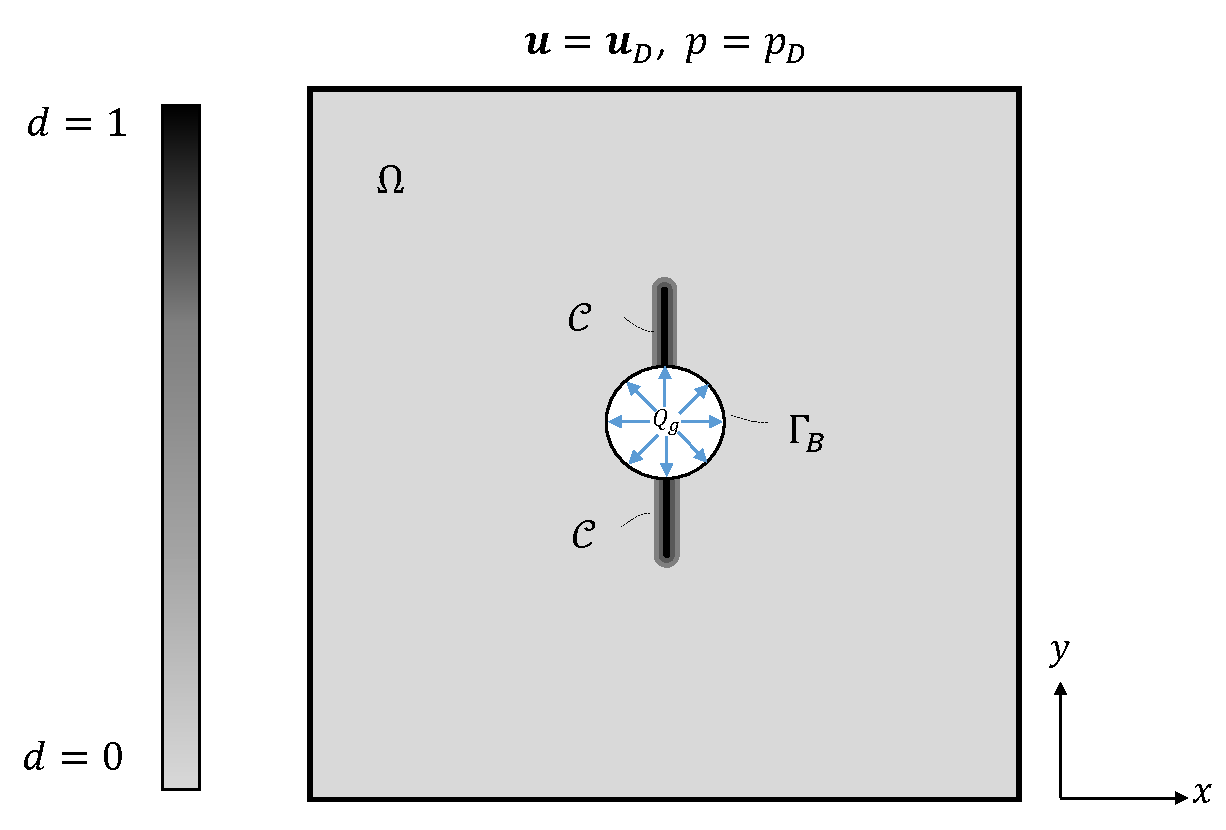
\includegraphics[width=0.8\textwidth]{omega_insitu2}
    \caption{Schematic of the computational domain. A square plate with a borehole placed inside is shown. The \emph{in situ} stress is applied on the external boundary, while the fluid is injected from the boundary of the borehole. The fracture $\mathcal{C}$ is approximated by a regularized crack surface $\mathcal{C}_{\ell}(d)$ which is a functional of the crack phase field.}
    \label{Fig:compute_domain}
\end{figure}

%\todo[inline]{YS: We have a conflict of notation for $\mu$. We need to use $G$ instead to represent the shear modulus.\\Vahid: Replaced.}

The variational approach to fracture is built on energy minimization with respect to the displacement field $\bm{u}:\Omega\rightarrow\mathbb{R}^2$ and its jump set, which we denote as $\mathcal{C}=\mathcal{C}(\bm{u})\subset\Omega$. Let $|\mathcal{C}|$ denote the one-dimensional Hausdorff measure of $\mathcal{C}$. Following Griffith's theory, the total potential energy of the fractured poroelastic solid is written as:
\begin{equation}\label{Eq:Pi}
    \begin{aligned}
        \Pi_{\mathcal{C}}[\bm{u},\mathcal{C}] &:= \int_{\Omega\setminus\mathcal{C}} \psi_0[\bm{\varepsilon}(\bm{u})] \; d\Omega
	    - \int_{\Omega} \bm{b} \cdot \bm{u} \; d\Omega
	    - \int_{\Gamma_N} \bm{t}_N\cdot \bm{u} \; d\Gamma \\
	    &- \int_{\Omega\setminus\mathcal{C}} \left(\alpha - 1\right)p\divergence\bm{u}\; d\Omega + 
	    \int_{\Omega\setminus\mathcal{C}}\nabla p\cdot \bm{u}\; d\Omega + g_c|\mathcal{C}|,\\
    \end{aligned}
\end{equation}
where $p$ denotes the pore pressure, $\alpha\in[0,1]$ is the Biot coefficient. {Constant} $g_c\in\mathbb{R}^+$ is the strain energy released per unit length of fracture extension. {The strain energy density $\psi_0[\bm{\varepsilon}(\bm{u})]$ is given by}
\begin{equation*}%\label{Eq:Strain_Energy}
    \begin{aligned}
        \psi_0(\bm{\varepsilon}) := \frac{\lambda}{2} (\trace \bm{\varepsilon})^2 + G \|\bm{\varepsilon}\|^2,
    \end{aligned}
\end{equation*}
with $\lambda$ and $G$ Lam\'e constants. These constants are related to Young's modulus $E$ and Poisson's ratio $\nu$ as $\lambda=E\nu/[(1+\nu)(1-2\nu)]$ and $G=E/[2(1+\nu)]$.
The linearized strain tensor takes the form:
\begin{equation*}
    \begin{aligned}
        \bm{\varepsilon}(\bm{u}) := 
        \frac{1}{2}\left(\nabla\bm{u}+\nabla\bm{u}^T\right).
    \end{aligned}
\end{equation*}
Finally, $\|\cdot\|$ denotes the Frobenius norm of a tensor.

\subsubsection{Regularized variational formulation of brittle fracture}
%\todo[inline]{YS: There is no need to explain $c_\omega$. Rather, its definition from $\omega(d)$ can be given instead. By the way, why $\omega$, not $w$?\\
%Vahid: I changed $\omega$ to $w$. Why not keeping the explanation of $c_w$? I kept it and also added its mathematical definition.}
%\Comment{YS: Do not use a backslash in the equation label.}
To develop a numerical method to approximate \eqref{Eq:Pi}, {the phase field approach replaces} the sharp-fracture description $\mathcal{C}$ with a phase field description, where the phase field is denoted as  $d:\Omega\rightarrow[0,1]$. In particular, regions with $d = 0$ and $d = 1$ correspond to the intact and fully broken materials, respectively. Using a phase field approach, the one-dimensional fracture $\mathcal{C}$ is approximated with the help of an elliptic %(Ambrosio-Tortorelli) 
functional \cite{ambrosio1990approximation, ambrosio1992approximation}:
\begin{equation}\label{Eq:Gamma_ell}
    \begin{aligned}
    \mathcal{C}_\ell[d]:=\frac{1}{4c_w}\int_\Omega\left(\frac{w(d)}{\ell} + \ell \nabla d\cdot\nabla d\right) d\Omega,  
    \end{aligned}
\end{equation}
where $\ell>0$ is the regularization length scale, which may also be interpreted as a material property, e.g., the size of the process zone. See Remark \ref{Rem:choice_ell} for comments on the choice of $\ell$. Constant $c_w=\int_{0}^{1} \sqrt{w(d)}$ is a normalization constant such that when $\ell\rightarrow 0$, {$\mathcal{C}_\ell[d]$} converges to the {length of the} sharp fracture{, $|\mathcal{C}|$}. Classical examples of $w(d)$ and $c_{w}$ are $w(d)=d^2$ and $c_{w}=1/2$ for the AT2 model, and $w(d)=d$ and $c_{w}=2/3$ for the AT1 model. Interested readers are referred to \cite{tanne2018crack,Bourdin2014014301} %\todo{YS: Wrong reference. The AT1 model came about in 2014 or so.\\Mostafa: Edited}~
for more elaborations.

%\todo[inline]{YS: We cannot use $\Pi$ for two different functionals. If the second one will be used more often, we can change the symbol for the first one, say $\Pi_{\text{sharp}}$.\\
%Vahid: Done. But the index `sharp' seems to me too long! I used $\Pi_{\mathcal{C}}$ instead. See \eqref{Eq:Pi}. Doesn't it look like better?}
%\todo[inline]{YS: See the new $\mathscr{S}_d$. I am still not clear about one thing: Do we impose $d\ge0$ or $d\ge$ its value at the previous time step?\\Vahid: OK. We impose $d\ge$ the previous value. The TAO solver gets a lower bound, and we update this bound every time step with the solution of $d$ from the last time step. Also, I changed $\mathscr{S}_d$ accordingly.}
On this basis, we replace \eqref{Eq:Pi} by a global constitutive dissipation functional for a rate independent fracture process \cite{BourdinCFRAC13}:
\begin{equation}\label{Eq:Dissipative_functional}
    \begin{aligned}
        \Pi[\bm{u},d] &:= \int_{\Omega} \psi[\bm{\varepsilon}(\bm{u}),d] \; d\Omega
	    - \int_{\Omega} \bm{b} \cdot \bm{u} \; d\Omega
	    - \int_{\Gamma_N} \bm{t}_N\cdot \bm{u} \; d\Gamma \\
	    &- \int_{\Omega}{\left(1 - d\right)}^2\left(\alpha - 1\right)p\divergence\bm{u}\; d\Omega + 
	    \int_{\Omega}{\left(1 - d\right)}^2\nabla p\cdot \bm{u}\; d\Omega \\
	    &+ \frac{g_c}{4c_{w}}\int_\Omega \left(\frac{w(d)}{\ell} + \ell \nabla d\cdot\nabla d\right)\;d\Omega,\\
    \end{aligned}
\end{equation}
where the admissible sets of displacement and phase field can be set as:
\begin{subequations}
\begin{align}
        \mathscr{S}_u &:= \left\{\bm{u} \in H^1\left(\Omega; \mathbb{R}^2\right) \middle|
        \bm{u} = \bm{u}_D \text{ on } \Gamma_D\right\}, \label{Su}\\
        \mathscr{S}_d &:= \{d\in H^1(\Omega)|0\le d\le 1\}.\label{Sd}
\end{align}
\end{subequations}
In practice, \eqref{Sd} will be used in combination with the irreversibility constraint, to be elaborated in Remark \ref{Rem:irreversibility}.
%\todo[inline]{YS: If we say ``Energy dissipation,'' then we have to give the dissipation rate. Otherwise we can say ``Degraded strain energy density'' or something of the sort.\\
%Vahid: I changed it to `Strain energy degradation'.}

%\todo[inline]{YS: Why not make these remarks as theorem-style environments? Then we do not need to number them by ourselves.
%\\ MM: I changed the style to theorem-style environment.}

%\todo[inline]{YS: The way I will organize the following paragraphs is perhaps first directly talk about Model A without mentioning even \eqref{Eq:psi}. Then Model B. As we do not have Model C here we do not need to be so general.\\
%Vahid: Following our discussion, I only kept the explanations for model B, now named as Amor's model.}

%\textsc{Remark 1} \textit{(Energy dissipation).}
%\todo[inline]{YS: See how I format the text that goes after ``Remark 1''}
\begin{remark}[Strain energy degradation]\label{Rem:psi}
The solid endures partial loss of stiffness due to the presence of fractures. In order to model this {effect}, the strain energy density is degraded with respect to the evolution of {the} phase field. Also note that as the damaged material responds differently to tension and compression, we let only a part of the strain energy density be degraded. For this purpose, we let the degraded strain energy in \eqref{Eq:Dissipative_functional} take the following general form:
\begin{equation*}%\label{Eq:psi}
\begin{aligned}
\psi(\bm{\varepsilon}, d) = g(d)\psi_+ + \psi_-,
\end{aligned}
\end{equation*}
where $g(d)$ satisfies $g(0)=1$, $g(1)=0$, and $g'(d)<0$ for all $d$ such that $0\le d\le 1$ \cite{Bourdin2000797}. A usual choice is $g(d)=(1-d)^2$. On the other hand, $\psi_{\pm}$ are such that
\begin{equation*}
    \begin{aligned}
        \psi_+(\bm{\varepsilon})+\psi_-(\bm{\varepsilon})=\psi_0(\varepsilon).
    \end{aligned}
\end{equation*}

Now since $\partial\psi/\partial d=g'(d)\psi_+$, only $\psi_+$ contributes to fracture propagation. 
\end{remark}

%\todo[inline]{YS: If we only do 3D or plane strain, we don't even need to mention what we do with the trace.\\
%Vahid: I omitted the relevant sentence. See below.}

%\deleted{Here we introduce two representative phase field models that differ in their choice of $\psi_+$.}

%\todo[inline]{YS: If we only use Amor \emph{et al.}'s model, we do not even need to say the name of the model.\\ Vahid: I deleted the relevant clause. See below}
There are several phase field models that differ in their choice of $\psi_{\pm}$. In this paper, we {adopt} the one proposed by Amor \emph{et al.}~\cite{Amor09}.
%\paragraph{Model A}
%\deleted{This is the original ''isotropic'' model \cite{Bourdin2000797}. It assumes the fracture responds similarly to tension and compression. It is convenient in that $\psi$ is continuous in both $\bm{\varepsilon}$ and $d$.}
%\paragraph{Model B} 
This model %\deleted{proposed by Amor \emph{et al.} \cite{Amor09}} 
assumes both volumetric expansion and deviatoric deformation contribute to fracture propagation, but volumetric compression does not. A decomposition of $\bm{\varepsilon}$ into volumetric and deviatoric parts reads:
\begin{equation*}
    \begin{aligned}
        \vol\bm{\varepsilon} := \frac{1}{3} (\trace\bm{\varepsilon}) \mathbf{1}, \quad
        \dev\bm{\varepsilon} := \bm{\varepsilon} - \vol\bm{\varepsilon}.
    \end{aligned}
\end{equation*}
%\deleted{where the trace operator is understood in three dimensions for both two-dimensional plane strain and plane stress cases.}

%\todo[inline]{YS: An alternative way to handle the irreversibility constraint is to use a history variable. Shall we mention it too?\\
%Vahid: I added a paragraph and mentioned this approach by Miehe as an alternative way.\\
%YS: Nice try, but it looks too long. We only need to say that a history field can be used for enforcing irreversibility. Moreover, although this point does not need to appear in the paper, the same concept of history variable can be used for Amor's model as well, without changing the way of tension-compression decomposition.\\
%Vahid: I have summarized the text now.}

%\textsc{Remark 2} \textit{(Irreversibility constraint).}

\begin{remark}[Irreversibility constraint]\label{Rem:irreversibility}
%With reference to \eqref{Eq:psi}, the minimum requirement on $g(d)$ is $g(0)=1$, $g(1)=0$, and $g'(d)<0$ for all $d$ such that $0\le d\le 1$ \cite{Bourdin2000797}. 
The requirement $g'(d)<0$ comes from the underlying irreversibility condition (the fracture can never heal) in time:
\begin{equation}\label{Eq:irreversibility}
    \partial_t d\geq 0.
\end{equation}
Consequently, modeling of fracture evolution problems leads to {inequality constraints, and sometimes gives rise to a variational inequality formulation}.

As an alternative way to {model} the irreversibility, Miehe \emph{et al.}~\cite{Miehe20102765} proposed a phase field model based on a local history field. In this model, the evolution of the phase field $d$ is driven by the historically maximum value of $\psi_+$ at the point of interest.
%{This model assumes that both volumetric expansion and deviatoric deformation contribute to the crack propagation but not volumetric compression.} 
%\added{In this model, the evolution of the phase field $d$ is defined as:}
%\begin{equation}\label{eq:18}
%\partial_t d=\frac{1}{\eta}\left\langle 2\left(1-d\right)H-\frac{g_c}{l}\left(d-l^2\Delta d\right)\right\rangle_+,
%\end{equation}
%\added{where $\eta>0$ is the \textit{artificial viscosity}, a material parameter to be input, $\langle a \rangle_\pm := (|a|\pm a)/2$ for all $a\in\mathbb{R}$, and}
%\begin{equation*}
%H(\bm{x},t) := \max_{s\in[0,t]} \psi_+(\bm{\varepsilon}(\bm{x})), \quad
%\psi_+(\bm{\varepsilon})= \frac{\lambda}{2} \langle \trace \bm{\varepsilon} \rangle_+^2 + \mu\sum_{i=1}^2 \langle\varepsilon_i\rangle_+^2
%\end{equation*}
%\added{is the historical maximum value of the tensile strain energy density of the point of interest.}
\end{remark}

%\todo[inline]{Vahid: I read somewhere by Bourdin \emph{et al.} that it has been shown the residual stiffness parameter $k$ has no significant impact on the numerical solution. Shall we omit this remark then?\\
%YS: If we used $k$, then just keep the remark. If not, then delete $k$ everywhere and this remark.}
%\begin{remark}[Residual stiffness]
%An additional small number $k$ with {$0<k\ll 1$} is added to the degradation function $g(d)$%coefficient of $\psi_+(\bm{\varepsilon})$
%, i.e., having $[(1-d)^2+k]$ instead of $(1-d)^2$ in \eqref{Eq:Dissipative_functional}, to prevent the lack of stiffness for completely fractured portions of the solid \cite{Bourdin2000797}. Here, we take $k=1\times10^{-12}$.
%\end{remark}
%\todo[inline]{
%YS: Equation \eqref{Eq:choice_ell} or something similar was proposed in 2014 by Bourdin.\\
%YS: I believe we should not stop here. We need to know what led to the two different expressions -- the different types of loading?\\Vahid: Now I find the formula by Bourdin \emph{et al.} \cite{Bourdin2014014301} suits more for our case, since it is for AT1 models in spite of the other work by Borden \emph{et al.} \cite{Borden2012A}. The details on how they end up with \eqref{Eq:choice_ell} is given in \cite{Bourdin2014014301}.\\
%Another point: As we have already defined $\lambda$ and $G$ at this point, we need to introduce $E$ in terms of $\lambda$ and $G$. Or we should have defined $\lambda$ and $G$ in terms of $E$ and $\nu$.
%\\Vahid: I put the conversion formula for $E$ in below.}
\begin{remark}[The choice of $\ell$]\label{Rem:choice_ell}
{Based on an analytical solution for the critical tensile strength $\sigma_\text{cr}$ that a one-dimensional bar can sustain \cite{Bourdin2014014301}, we use the following equation for the choice of $\ell$:}
\begin{equation}\label{Eq:choice_ell}
    \begin{aligned}
        \ell=\frac{3Eg_c}{8\sigma_\text{cr}^2},
    \end{aligned}
\end{equation}
where $E$ and $g_c$ can be obtained from regular experiments, while $\sigma_\text{cr}$ can be approximated by the tensile strength $\sigma_t$. Assuming all {other} parameters are known, the formula \eqref{Eq:choice_ell} is able to estimate $\ell$, though the accuracy is unknown for more complex cases.
\end{remark}
%\todo[inline]{YS: Maybe we don't need this subsubsection at all.\\Vahid: Or shall we move it to \ref{sub:weak_form}?\\
%YS: The problem with the EL equations is that they hold only when the equality holds, while we are solving a constrained minimization problem. Wherever the constraint $d\le 0$ or $d\ge 1$ is in place, the corresponding EL \eqref{Eq:Euler_d} does not holds.
%\\Vahid: OK. So the EL subsection does not exist anymore.}
%\subsubsection{The Euler-Lagrange equations}
%%\todo[inline]{YS: These spaces should be introduced as constraints for the optimization problem with \eqref{Eq:Dissipative_functional}.
%%\\Vahid: Now they are placed right after \eqref{Eq:Dissipative_functional}.}
%
%%\todo[inline]{YS: I got $-\mathbf{b}$ instead of $\mathbf{b}$ in \eqref{Eq:Euler_u}.\\
%%Vahid: Correct. Not it's changed.}
%
%The Euler-Lagrange equations of \eqref{Eq:Dissipative_functional} are obtained by {taking} the first variations with respect to $\bm{u}$ and $d$ {followed by appropriate integrations by parts}, and are expressed as follows:
%\begin{subequations}\label{Eq:Euler}
%    \begin{align}
%         \label{Eq:Euler_u}  {-}\divergence\bm{\sigma} - \mathbf{b} +
%        \left(\alpha-1\right) \nabla  \left[ (1-d)^2 p\right] + \left(1-d \right)^2 \nabla p &= \mathbf{0}, \quad  \text{in~} \Omega, \\
%        \label{Eq:Neu_u} \bm{\sigma}\cdot\bm{n} - \bm{t}_N &= \bm{0}, \quad \text{on~} \Gamma_N, \\
%        \begin{split}
%                  \label{Eq:Euler_d} \frac{\partial\psi}{\partial d} + \frac{g_c}{4c_{w}\ell}\left({w}'(d) - {\ell}^2 \Delta d\right)
%        + 2 \left(\alpha-1\right) \left(1-d \right)p\divergence \bm{u}
%        \\- 2\left(1-d\right)\nabla p\cdot\bm{u} &= 0, \quad  \text{in~} \Omega, 
%        \end{split}
%          \\
%        \label{Eq:Neu_d} \frac{\partial d}{\partial \bm{n}} &= 0, \quad  \text{on~} \partial\Omega,
%    \end{align}
%\end{subequations}
%where
%\begin{equation*}
%    \begin{aligned}
%        \bm{\sigma} =\frac{\partial\psi}{\partial\bm{\varepsilon}} = g(d) \bm{\sigma}_+(\bm{\varepsilon}) + \bm{\sigma}_-(\bm{\varepsilon})
%    \end{aligned}
%\end{equation*}
%is the Cauchy stress with $\bm{\sigma}_\pm(\bm{\varepsilon}):=\partial\psi_\pm/\partial\bm{\varepsilon}$, and $\bm{n}$ is the unit outer normal to $\partial\Omega$. Here \eqref{Eq:Euler_u} expresses the momentum conservation of the solid, \eqref{Eq:Euler_d} defines the phase field evolution, and \eqref{Eq:Neu_u} and \eqref{Eq:Neu_d} are Neumann boundary conditions for $\bm{u}$ and $d$, respectively.

\subsection{Carbon dioxide as a compressible fluid} \label{Sec:CO2}
The governing equations for the fluid flow in a porous medium are given by mass conservation, momentum balance, and the equation of state.
The mass conservation equation reads:
\begin{equation}\label{Eq:Mass_Conserv}
    \begin{aligned}
        \partial_t\left(\phi\rho\right)  +\nabla\cdot\left(\rho\bm{q}\right)&=0  \quad  &\text{in~} \Omega, \\
    -\rho\bm{q} \cdot n &=Q_g  \quad  &\text{on~} \Gamma_B.       
    \end{aligned}
\end{equation}
Here $\phi$ denotes the porosity of the porous medium (the fraction of volume occupied by the fluid), $\rho$ the density of the fluid, $\bm{q}$ the Darcy velocity vector, and $Q_g$ the fluid source. Note that $Q_g$ has the unit of volumetric flow rate per unit volume. Also, we assume the rock is saturated by the fluid so that the fluid content in rock per volume is expressed by $\phi\rho$.

%\todo[inline]{YS: Do we have the last term of \eqref{Eq:Darcy_law} in the numerical model or not? If not, then we do not need it in the equation, just mention it in the text.\\
%Vahid: No, we don't use this term. I deleted it then. I prefer we even not mention it in the text, as some other references do. Now I mentioned it though. See below.\\
%YS: Is it because $z$ is the direction perpendicular to our plane of interest? If so, it is easy to justify.\\Vahid: Yes, it is.}

In addition to \eqref{Eq:Mass_Conserv}, we state the momentum balance in the form of Darcy's law. This law indicates a linear relationship between the fluid velocity and the head pressure gradient:
\begin{equation}\label{Eq:Darcy_law}
    \begin{aligned}
        \bm{q} = -\frac{k}{\mu} \nabla p,
    \end{aligned}
\end{equation}
where $k=k(d)$ is the permeability of the rock, and $\mu$ is the dynamic fluid viscosity. %\replaced{}{$g$ is the magnitude of the gravitational acceleration, and $z$ is the depth} 
Note that there could be an additional term $- \rho g\nabla z$ %\todo{YS: $\nabla z$? It is a valid definition but $\nabla z=\bm{e}_z$ (the unit vector in the $z$-direction. Is it just $z$?)\\Vahid: I believe it is $\nabla z$, and since in our case $|\nabla z|=1$, hence $\rho g \nabla z$ is much smaller than the magnitude of the other vector, i.e., $\nabla p$.} 
on the right hand side of \eqref{Eq:Darcy_law}, where $g$ and $z$ are the magnitude of the gravitational acceleration and the depth, respectively. This term is, however, in our case negligible, as we assume an almost horizontal computational domain.
%Note the effect of the second term ($\rho g\nabla z$) is negligible.
Also, we assume the porosity is not dependent on the stress condition. On the other hand, we correlate the permeability to the phase field value by:
\begin{equation}\label{Eq:k_0}
    \begin{aligned}
        k(d) = k_0\exp{\left({\alpha}_k d\right)},
    \end{aligned}
\end{equation}
where $k_0$ is the permeability of the intact material, and ${\alpha}_k$ is a coefficient to indicate the effect of phase field evolution on the permeability. We take ${\alpha}_k=7.0$ (see \cite{PILLAI201836, ZHU2013179} for more description). Figure \ref{Fig:Permeability_increments} illustrates the permeability increasing with respect to the evolution of the phase field variable.

%\todo[inline]{YS: How about changing the vertical axis of Figure \ref{Fig:Permeability_increments} to $k(d)$?\\Mostafa: Done.}

\begin{figure}[htbp]
    \centering
    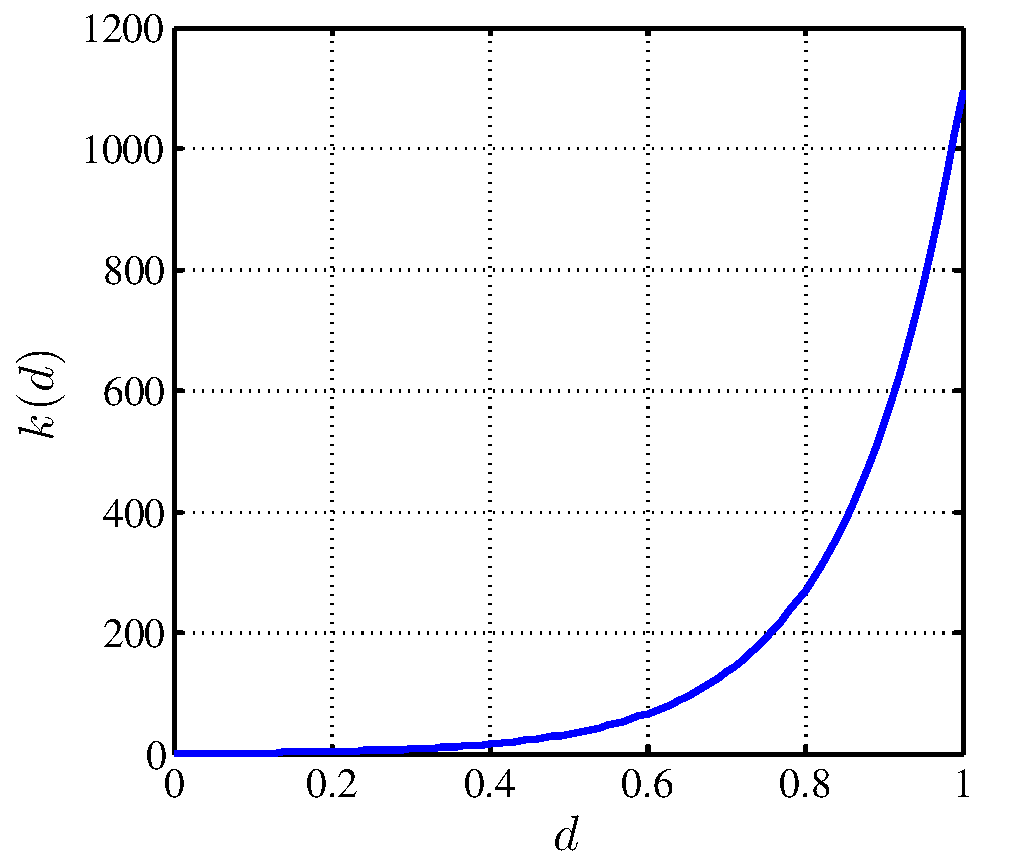
\includegraphics[width=0.6\textwidth]{permeability}
    \caption{Plot of $k(d)=\exp(7.0 d)$, permeability, as a function of the phase field variable $d$.}
    \label{Fig:Permeability_increments}
\end{figure}

The first term on the left hand side of \eqref{Eq:Mass_Conserv}, the rate of change of fluid content, can be written as:
\begin{equation}\label{Eq:diff_m}
    \begin{aligned}
        \partial_t\left(\phi\rho\right) = \rho \; \partial_t \phi +\phi \; \partial_t \rho  = \rho \;  \partial_t \varepsilon_v{+\phi \; \partial_t \rho},
    \end{aligned}
\end{equation}
where we have assumed the rate of change of pore volume is equal to that of the volumetric strain, which is given by $\varepsilon_v= \nabla \cdot \bm{u}$. 

%\todo[inline]{YS: I find the derivation of \eqref{Eq:Darcy_right} is exact. Where did we neglect the quadratic gradient term? Or \emph{will} we? Then we need to add one more step with $\doteq$ or $\approx$ at the end.\\
%Vahid: Yes, the derivation was exact. I also added the approximation to the equation. But note in the implementation/code, we neglect the quadratic term. I changed the text and equation accordingly.\\
%YS: But the exact derivation would have a term with $\nabla k$, or equivalently, $k'(d)\nabla d$.\\
%Another point: What is the justification for us to neglect the quadratic term? Is it because $p$ is the fluctuation value above some constant reference value?\\Vahid: Finally we came up with \eqref{Eq:General_pressure}.}

%\todo[inline]{YS: Shall we multiply \eqref{Eq:Darcy_right} by $-1$?\\Vahid: Not existed anymore.}
%\deleted{Also, with \eqref{Eq:Darcy_law}, the first term of the right hand side of \eqref{Eq:Mass_Conserv} is computed as:}
%\begin{equation}\label{Eq:Darcy_right}
%    \begin{aligned}
%        \nabla\cdot\left(\deleted{-}\rho\frac{k}{\mu}\nabla p\right) = \nabla\left(\deleted{-}\rho\frac{k}{\mu}\right)\cdot\nabla p  \replaced{+}{-} \rho\frac{k}{\mu}\Delta p &= \deleted{-}\frac{k}{\mu}\left[ \frac{d\rho}{dp} \left|\nabla p\right|^2 + \rho \Delta p\right]\\&\doteq\deleted{-}\frac{k}{\mu}\rho\Delta p
%    \end{aligned}
%\end{equation}
%\begin{equation}\label{Eq:Darcy_right}
%\begin{aligned}
%\nabla\cdot\left(\deleted{-}\rho\frac{k}{\mu}\nabla p\right) = \nabla\left(\deleted{-}\rho\frac{k}{\mu}\right)\cdot\nabla p  \replaced{+}{-} \rho\frac{k}{\mu}\Delta p &= \deleted{-}\frac{k}{\mu}\left[ \frac{d\rho}{dp} \left|\nabla p\right|^2 + \rho \Delta p\right]+\added{\frac{\rho}{\mu}\nabla k\cdot\nabla p}\\&\deleted{\doteq\deleted{-}\frac{k}{\mu}\rho\Delta p}
%\end{aligned}
%\end{equation}
%\begin{equation}%\label{Eq:Darcy_right}
%    \begin{aligned}
%        \nabla\cdot\left(-\rho\frac{k}{\mu}\nabla p\right) = \nabla\cdot\left(-\rho\frac{k}{\mu}\right)\nabla p  - \rho\frac{k}{\mu}{\nabla}^2 p = -\frac{k}{\mu}\left[ \frac{d\rho}{dp} \left(\nabla p\right)^2 + \rho{\nabla}^2 p\right]
%    \end{aligned}
%\end{equation}
%\deleted{Note that for sake of simplicity, {in our implementation} we neglect the quadratic gradient term of pressure $|\nabla p|^2$ {in \eqref{Eq:Darcy_right}}.
%}
%\todo[inline]{YS: There are many parameters like $d_i$, $t_i$, etc., undefined in \eqref{Eq:Res_Helmholtz}. Maybe we can say they are given in \cite{span1996new}.\\ Vahid: We already referred the readers for the many parameters. See ``Interested readers\dots'' now in blue.\\
%YS: Well, not just interested readers. The information is not complete for readers to reproduce our results. We need to give the numbers of all these parameters. Explanation is optional, though.\\Vahid: How does it look like now?}

Under isothermal conditions, the gas density varies significantly with pressure. This is {captured} by an equation of state (EOS). One applicable EOS for CO$_2$ is known as the Span-Wagner (S-W) equation \cite{span1996new} defined in terms of the Helmholtz free energy. The CO$_2$ density and pressure are related by:
\begin{equation}\label{Eq:Density_Pressure}
    \begin{aligned}
        p=\left(1+\delta\varphi^r_{\delta}\right)\rho RT,
    \end{aligned}
\end{equation}
where $R$ is the universal gas constant, and $\varphi^r_{\delta}$ is the derivative of the residual part of the full expression of Helmholtz energy $\varphi^r$ with respect to the reduced density $\delta$, with %. It is written as:
\begin{equation}\label{Eq:Res_Helmholtz}
    \begin{aligned}
        \varphi^r\left(\delta,\tau\right) &= \sum_{i=1}^{7} n_i  \delta^{d_i}\tau^{t_i}+\sum_{i=8}^{34} n_i\delta^{d_i} \tau^{t_i} e^{-\delta^{c_i}}+ \sum_{i=35}^{39} n_i  \delta^{d_i}\tau^{t_i} e^{-\alpha_i\left(\delta-\varepsilon_i \right)^2-\beta_i\left(\tau-\gamma_i\right)^2}\\ &+\sum_{i=40}^{42} n_i\Delta^{b_i}\delta e^{C_i\left(\delta-1\right)^2-D_i\left(\tau-1\right) ^2},\\
    \end{aligned}
\end{equation}
in which
\begin{equation*}\label{Eq:Delta}
    \begin{aligned}
        \Delta=\left\lbrace\left(1-\tau \right)+A_i\left[\left(\delta-1 \right)^2\right]^{\dfrac{1}{2\beta_i}}\right\rbrace ^2+B_i\left[\left(\delta-1 \right)^2\right]^{a_i}.
    \end{aligned}
\end{equation*}
In \eqref{Eq:Res_Helmholtz}, $\rho_c$ and $T_c$ are the critical density and temperature, respectively, and $\delta=\rho/\rho_c$ and $\tau=T/T_c$ are the reduced ones. For the sake of brevity, here we do not provide the definitions and values of other parameters in \eqref{Eq:Res_Helmholtz}, but refer the readers to \cite{span1996new}.

%\todo[inline]{YS: It looks more natural for \eqref{Eq:Density_Pressure} to come before \eqref{Eq:Res_Helmholtz}, otherwise it seems a puzzle why we need the latter.\\Mostafa: Done}

%\todo[inline]{YS: ``$\delta \varphi^r_{\delta}$ and $\delta^2 \varphi^r_{\delta \delta}$ are the first and second derivatives of $\varphi^r$ with respect to $\delta$, respectively'' seriously? It looks like $\varphi^r_{\delta}$ and $\varphi^r_{\delta \delta}$ are the first and second derivatives of $\varphi^r$ with respect to $\delta$, respectively. By the way, why do we keep the superscript $r$ all along?\\
%Vahid: You're right about the derivatives of $\varphi^r$. I changed the text accordingly. Regarding the superscript $r$, as we denote by $\varphi^r$ the `residual' part, I preferred to keep it. And also it is easier for the reader to follow as she finds the same notation in other references.}

%\todo[inline]{YS: Is $k/\mu$ constant or not? I felt the derivation of \eqref{Eq:Darcy_right} can only go through in the case of yes. Then in \eqref{Eq:General_pressure} why did we move it back inside the parentheses instead of writing $-(k/\mu) \Delta p$?\\
%Vahid: Actually no. $k/\mu$ is not constant as $k$ is a function of $d$. However, I find that the derivation of \eqref{Eq:Darcy_right} is still correct. I put $-(k/\mu)\rho\Delta p$ in \eqref{Eq:General_pressure}.}

By substituting  \eqref{Eq:Darcy_law},\eqref{Eq:k_0}, \eqref{Eq:diff_m}, and \eqref{Eq:Density_Pressure} in \eqref{Eq:Mass_Conserv}, the governing equation for CO$_2$ flow is written as follows: 
%\begin{equation}\label{Eq:General_pressure}
%    \begin{aligned}
%        \frac{\phi}{{N}} \partial_t p +\rho \; \partial_t \varepsilon_v -\frac{k}{\mu}\left[\frac{d\rho}{dp}\rho\Delta p\right] =Q_g,
%    \end{aligned}
%\end{equation}
\begin{equation}\label{Eq:General_pressure}
\begin{aligned}
\phi \; \partial_t \rho+\rho \; \partial_t \varepsilon_v -\nabla \cdot \left( \rho \frac{ k(d)}{\mu} \nabla p \right) =0,  \quad  &\text{in~} \Omega,\\
    \rho\bm{q} \cdot n =-Q_g,  \quad  &\text{on~} \Gamma_B,\\
    p = p_D, \quad &\text{on~}\Gamma_P,
\end{aligned}
\end{equation}
where $\Gamma_P=\partial\Omega\setminus\Gamma_B$. 
%\todo[inline]{YS: If the fluid is incompressible, then we should have $K_f=\infty$, right?\\
%Vahid: Yes.\\
%YS: Then why do we not take away the term $\phi/K_f$ as it vanishes?\\
%Vahid: We finally agreed to delete this part.}
%In the rock mechanics, we usually use the mulation of Detournay \cite{detournay1995fundamentals} (Table 2, page 123) related to "\textbf{Invariance of porosity under $\Pi$-loading}"   while for "\textbf{Incompressible fluid and solid constituents}" (page 122) you are right $K_f \rightarrow \infty$ }

%\paragraph{\deleted{Incompressible fluid flow}} \deleted{Here, it is also worth mentioning the case of incompressibility. For the incompressible fluid flow, the left-hand-side of \eqref{Eq:Mass_Conserv} reads} \cite{detournay1995fundamentals}:
%\begin{equation}\label{Eq:Mass_Left}
%    \begin{aligned}
%       \deleted{ \partial_t \left(\phi\rho\right) =
%        \phi \; \partial_t  \rho+ \rho \; \partial_t \phi
%        = \rho\left(\frac{\phi}{K_f}+\frac{\alpha -\phi}{K_s}\right)
%       \partial_t p + \alpha\rho \;  \partial_t \varepsilon_v,}
%    \end{aligned}
%\end{equation}
%\deleted{where $K_f$, $K_s$ are the bulk modulus of fluid and rock grains, respectively. 
%Combining Eqs.~\eqref{Eq:Mass_Conserv}-\eqref{Eq:Mass_Left}, the generalized equation of the incompressible fluid flow is obtained as follows:}
%\begin{equation}\label{Eq:Mass_General}
%    \begin{aligned}
%        \deleted{\left(\frac{\phi}{K_f}+\frac{\alpha -\phi}{K_s}\right) \partial_t p+  \alpha \; \partial_t \varepsilon_v+\nabla \cdot \left( -\frac{k}{\mu}\nabla p\right) =Q_g.}
%    \end{aligned}
%\end{equation}

%\todo[inline]{YS: Here we need to summarize a non-redundant collection of equations.\\Vahid: Added below.\\
%YS: It is still not clear that for the solid it is a constrained minimization problem.\\Vahid: More descriptions are added now.}
%\todo[inline]{YS: Comparing $\mathscr{S}_p$ and $\mathscr{S}_u$, does it mean $p$ and $\bm{u}$ will always be imposed on the same part of $\partial\Omega$, called $\Gamma_D$? By the way, why do we need the admissible pressure for the strong form? I added the corresponding boundary condition instead. Please confirm.\\Vahid: Now I defined $\Gamma_P$ for $p_D$. The admissible pressure is moved to \ref{sub:weak_form}.}
\paragraph{Summary of governing equations} The governing equations for modeling the CO$_2$ fracturing are summarized as follow: for the porous medium deformation, the functional defined in \eqref{Eq:Dissipative_functional} is minimized among $(\bm{u},d)\in \mathscr{S}_u\times\mathscr{S}_d$ under the constraint \eqref{Eq:irreversibility}, while %The lower bound $d^{n-1}$ is considered to ensure the irreversibility of the fracture. 
for the compressible fluid the boundary value problem \eqref{Eq:General_pressure} is used to solve for the pressure $p$.

Note also that $d\equiv0$, i.e., there is no preexisting crack in the specimen and we do not allow for any nucleation of the fracture as the rock strength is assigned a very large value.
